\chapter{Client-Side JS: Sound \& Vision APIs}
\label{sound-and-vision}
\paragraph{} Just like in the last topic where we looked at the data storage APIs of the browser, in this unit we focus upon a specific set of APIs for doing things with audio (sound) and with graphics (vision). Basically we can use the browser's sound and vision JS APIs to create awesome experiences for our users that go way beyond text presentation.
\paragraph{} Be aware though that each of these topics is very large and could conceivably constitute an entire module individually, so what we'll study here is merely an overview and a taster of what can be done. Practically, the only limitation in sound and vision is your imagination, because the tools that the sound and vision APIs gives us are very powerful, ultimately enabling us to create raw sounds by manipulating frequency and waveform, and to create images by placing individual pixels.
\paragraph{} We'll deal with each sub-topic individually, starting with sound and then moving on to vision.

\section{Sound}

\paragraph{} Sound in the Web browser is handled through the Web AudioContext object. Really the web browser, your operating system, and your hardware are handling much of the task, acting to turn your instructions into perceivable reality. The AudioContext object is our interface to the sound related features that the browser provides, and also gives us a theoretical model, based on graphs, for creating, manipulating, and outputting sounds.

\paragraph{} Our browser provides basic functionality for:

\begin{itemize}
\item Playing sound files (Audio Playback)
\item Creating sounds from scratch (Audio Synthesis)
\end{itemize}

\paragraph{} We'll look at each in turn, starting with playing back existing sound files, then looking at how to create sound signals from scratch by synthesising the sound waves that make up the sound.

\section{Playing Audio Files}

\paragraph{} If we’ve already got an audio file, i.e. we don't need to synthesise any new audio then we can just play that audio as is. To enable this we can use the MP3, Ogg, and Wav formats which are supported as standard.
\paragraph{} To play a file we merely use the HTML5 <audio> element which supports, by default, the MP3, Ogg, and Wav formats. Basically all we have to do to play an existing file in a web page is to include the audio element. This is just like how if we want to include a picture on a web page we include the <img> element. So audio gets treated as though it is a distinct entity within our web page. This also means that it is exposed via the DOM to JS, so we can manipulate our audio element, but more about that later.
\paragraph{} The audio element has a variety of attributes that we can set and manipulate which give us, and our users, some control over the resulting audio playback. For example, the controls attribute gives our users a set of shuttle controls and other user interface elements for interacting with the audio. This can include playing and stopping the audio, and moving the current playback position within the file. We can also set other attributes such as autoplay and muted. Note that autoplay is frequently prohibited in many modern browsers, requiring some user interaction with the page before play begins. As a result you shouldn't rely on the ability to autoplay an audio file when your page loads as part of your user experience. However you can have audio playback autostart at page load time, but only if the sound is muted.

\section{An $<$audio$>$ example}

\paragraph{} Let's first look at how to include the audio element within a simple HTML web page. 

\begin{lstlisting}
<!DOCTYPE html>
<html>
    <body>
        <audio id="my_audio_control" autoplay loop controls>
            <source src="horn.mp3" type="audio/mpeg">
            Your browser does not support the audio element.
        </audio>
    </body>
</html>
\end{lstlisting}

\paragraph{} Notice that we have set the autoplay, loop, and controls attributes. We tell the audio control what to play by providing a <source> element defining both the location of the file to play and its type. We also added a message to display if the browser that is viewing this page does not support the <audio> element. The result is shown in the following screen capture. You should experiment with different combinations of attributes to get a feeling for how this element works.

\begin{figure}[H]
\centering
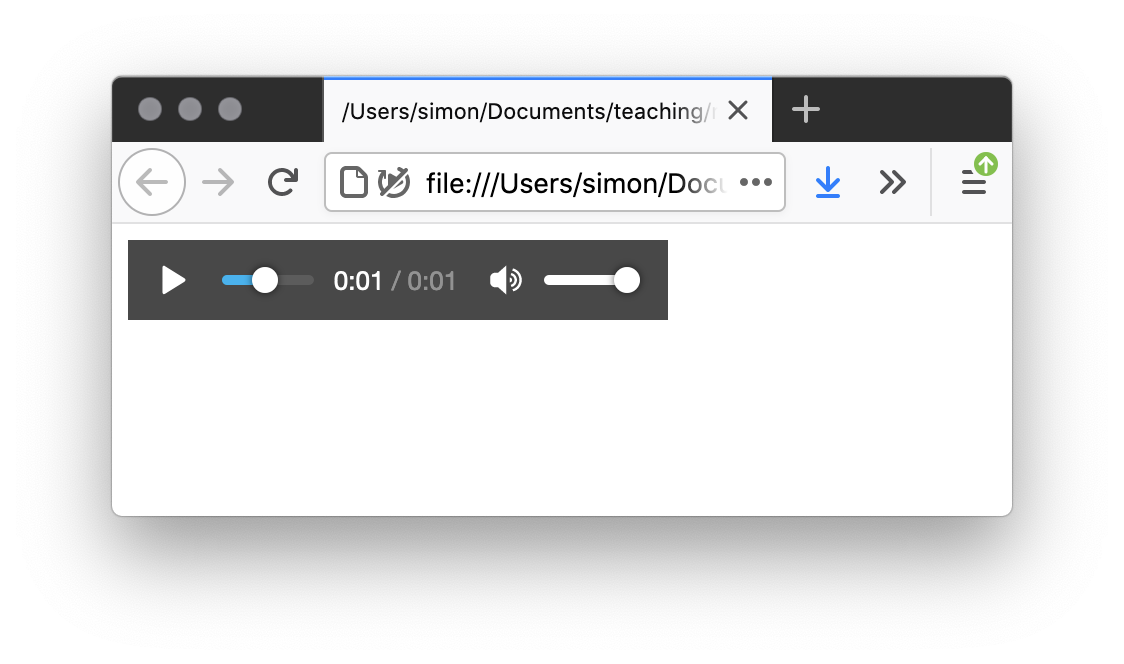
\includegraphics[width=0.8\textwidth]{figures/audio-ui}
\label{fig:audio-ui}
\caption{}
\end{figure}

\section{Interacting with $<$Audio$>$ from JS}
\paragraph{} In the last example we relied upon our user to control the playback of our audio files. For many circumstances this is perfectly fine. When we combine this with the ability to use CSS to style the presentation of the audio element we can build user interfaces that naturally integrate the audio playback amongst our other features. However, the degree to which this can be controlled in a reliable way is currently uncertain. Many of the styling options are available through the webkit pseudo extensions and thus may be subject to change in the details of how they function.
\paragraph{} However this does raise an interesting point. We can set the hidden attribute to hide the player, or else we can set the controls attribute to false from JS which also hides the player, in both cases causing the audio controls to be hidden. This effectively removes control of the audio from most users, but is problematic from a usability and user experience perspective. Without audio controls the user can't stop annoying audio from playing, or has to use the system sound settings to adjust sound levels, so what is the solution if we don't want to expose the standard audio controls to our users but do want to give them a good user experience? The answer, as with many aspects of web development, is to use HTML, and especially JS, to build alternative interface elements.
\paragraph{} Let's look at a simple example of that now:

\begin{lstlisting}
<!DOCTYPE html>
<html>
    <body>
        <audio id="my_audio" autoplay="autoplay" loop controls>
            <source src="horn.mp3" type="audio/mpeg">
            Your browser does not support the audio element.
        </audio>
        <button onclick="toggle_loop()" type=“button">Toggle looping</button>
        <script>
            var ao = document.getElementById("my_audio");
            function toggle_loop() {
                if (ao.loop) { ao.loop = false; }
                else { ao.loop = true; }
                ao.load();
            }
        </script>
    </body>
</html>
\end{lstlisting}

\paragraph{} In this example, we’ve merely added a button to control whether the audio loops, but the method is similar for controlling other aspects of the audio element. Although we've kept the standard user interface displayed, once we have a critical mass of functionality provided through our own user interface elements, at least so the user can start and stop audio playback, then we will be in a position to hide the default audio controls and offer only those which fit with our designs.
\paragraph{} Interacting with other attributes through JS happens in a similar fashion. You can use the HTML standard\footnote{\url{https://developer.mozilla.org/en-US/docs/Web/API/HTMLAudioElement}} to investigate the remaining attributes and their legal values, but these include volume, loop, muted, controls, as well as methods such as play(), and pause().
\paragraph{} Note that because the audio element is a child of the more general HTMLMediaElement, playback control methods are provided by that element rather than by the audio element itself, so we have to look to the media element API\footnote{\url{https://developer.mozilla.org/en-US/docs/Web/API/HTMLMediaElement}} for those parts.
\paragraph{} You should now be able to build your own user interfaces to enable your users to control playback of existing audio files within your sites.


\section{Audio Synthesis}
\paragraph{} So far we've only considered playing back existing audio from MP3 or similar media files using the <audio> element. However we have a much more powerful mechanism available to us for working with audio. Rather than playing back existing sounds e.g. from music files, we can create sound, from first principles, using JS. This means that instead of recording a real sound, a similar, or completely different sound can be artificially constructed by using the right values for the components of the sound. We'll refer to this process as audio synthesis.
\paragraph{} For several decades synthesisers have been electronic musical instruments, frequently seen in piano keyboard form, but they do a similar function to what we will do using the JS AudioContext. Both are technically synthesisers, they allow us to create sounds by manipulating the components of sound, to get the effect that we want.
\paragraph{} Note that the idea of ``getting the effect that we want'' should raise the idea in your mind that creating the audio for your site is as much about designing a user experience as any other part of web design, such as designing the visual, or interactive experience.


\section{What is Sound?}
\paragraph{}
Before we can get to grips with what AudioContext can do for us, we first need to turn our attention to the nature of sound. This is because AudioContext is built around a fundamental understanding of what sound is and how it works. By understanding this, we provide ourselves with a theoretical framework in which the operation of AudioContext makes more sense. Let's start with a working definition of sound:
\begin{verbatim}
Sound is a Movement (vibrations/oscillations) that travels (acoustic wave) through a medium (usually air) that can be perceived (detected/heard) when they reach a sensor (ear/microphone)
\end{verbatim}
\paragraph{} The character of any given sound is affected by a lot of factors, but there are some fundamental features that have a great effect upon the resulting sound. These are:

\begin{itemize}
\item The shape of the wave. In audio synthesis we usually consider four core shapes, known as waveforms. These include the sine wave, the square wave, the triangle wave, and the sawtooth wave. We can also create custom waveforms by supplying sine and cosine values to a PeriodicWave node, but for our purposes we'll stick with the four builtins.
\item We're only going to consider periodic waveforms, that is waveforms that repeat continuously until the sound stops. How often the repetition occurs is called the frequency of the wave. The frequency is usually defined in terms of the number of times, that is the number of cycles, that the wave repeats per second. Such measurements are made in Hertz (Hz) where 1Hz is defined as 1 cycle per second. Humans can generally hear sound that vibrates in the range between 20Hz and 20kHz, that is between twenty times per second and twenty thousand times per second. As we age our ability to hear at the extremes of these ranges, particularly at higher frequencies, is curtailed.
\item Amplitude is a measure of how much any given wave changes during a cycle. Think of waves on a beach and consider the distance from the normal water level to the top of a wave (and also conversely the distance from normal water level to the bottom of the trough between waves). Amplitude for any given wave is a measure from the normal level, i.e. the midpoint between peaks and troughs, to the top, or bottom, of a wave. In audio synthesis we'll use amplitude as a proxy for loudness, but in reality loudness is really more complex and involves also the power (or intensity) of the sound. For our current purposes though, amplitude is a useful proxy for loudness.
\end{itemize}

\paragraph{} We'll see that many aspects of sound depend upon this simple understanding of sound. A speaker, such as that on a radio, creates sound by turning a signal (which can be analogue or digital) in to a set of vibrations. This is achieved by moving at various frequencies and amplitudes, which in turn causes air to move, which our ears subsequently detect and our brains interpret. Conversely, a microphone is very similar to a speaker in inverse, a device that detects vibrations and returns them to a signal, initially analogue and then often converted into a digital audio signal. 
\paragraph{} Similarly, within a browser we can create audio by generating sound waves. A computer can control the frequencies and amplitudes (and other things) of multiple simultaneous sound waves to enable the resulting generated sound to make sense to us or otherwise fulfil the purpose that the sound is designed for. For example we might want to generate audio that sounds like something, that forms music, or is recognisable as a voice, or some other recognisable noise like thunder, or that we react to, like a siren.

\section{The AudioContext \& Browser Audio}
\paragraph{} Sound synthesis in the browser focuses on the construction of an audio-processing graph.
\paragraph{} Remember: A graph is a mathematical model that is constructed from nodes that are connected to each other by edges. This basic idea is used in lots of ways throughout computing for modelling various ideas. Sound modelling is just one way to use graphs.
\paragraph{} An AudioContext is just a graph that links audio processing modules (AudioNode) together. We create an AudioContext, which is an empty graph. We then add nodes to this graph to represent parts of our audio signal, from its creation, through any processing to change how it sounds, through to its destination, i.e. output via speakers to our ears.
\paragraph{} Usually we would create a single AudioContext that we then reuse as needed in our site, e.g.

\begin{lstlisting}
var audioCtx = new AudioContext();
\end{lstlisting}

\paragraph{} In practice though, because of differences between browsers in how the audio API is implemented, we often need to use the following to create an AudioContext:

\begin{lstlisting}
var audioCtx = new (window.AudioContext || window.webkitAudioContext)();
\end{lstlisting}

\paragraph{} This becomes our handle to the audio context that we can manipulate and control via JS. An important property of the AudioContext object is the destination which is the place that sounds are output to (usually the computer speaker). We usually need to specify the destination to use once we've created an AudioContext otherwise we won't hear anything because there won't be an output.
\paragraph{} We can create Audio Nodes and then connect them into our audio processing graph, represented by our AudioContext. These Audio Nodes create and shape the sounds we hear at the destination as the sounds pass through the graph. It can be useful to think of this process as a bit like sending water through pipes. Water can be diverted and made to run through various processes, perhaps UV treatment and particulate filtering, with the result being clean drinking water. Audio moving through an AudioContext graph is very similar, it can be filtered and manipulated so that what comes out at the destination is very different to what would be heard at the starting place. It is the filtering and manipulation process that we can use to our advantage to create the sounds that we want our users to hear.


\section{Creating a Sound}
\paragraph{} Let's see how all of this comes together. We need to create an audio context graph, then add a sound source node to our graph, connect that sound source to a destination, and then get it to start sounding.
\paragraph{} The starting place for sounds is an oscillator (these create vibrations so are the starting place for synthesising sounds). Remember back to our discussion of speakers earlier, the speaker's cone is an oscillator that responds to a signal, it then moves back and forth, it oscillates. Within our AudioContext, an oscillator is very similar, whilst it doesn't physically move, it digitally captures the idea of a starting place for our sound, something that moves backwards and forwards at a given frequency. How about the musical note ‘A’, that has a known frequency value of 440Hz. This is the default value for an oscillator but we're going to set it explicitly in our next example to show how to do that (and also to give you an opportunity to explore different frequencies).
\paragraph{} You can type the following directly into your browser's web console (shortly we'll see how to embed this into a web page though as well):

\begin{lstlisting}
var context = new (window.AudioContext || window.webkitAudioContext)();
var oscillator = context.createOscillator();
oscillator.frequency.value = 440;
oscillator.connect(context.destination);
oscillator.start();
\end{lstlisting}

\paragraph{} Here we've create an AudioContext that we've assigned to the 'context' variable. We've then created an oscillator, which we've assigned to the 'oscillator' variable. We've then set the frequency value for the oscillator to 440Hz. To form our graph we need to connect our oscillator to something. As we don't need to do anything more to process our sound, we now merely connect our oscillator to our browser's default destination and the set it to start.

\paragraph{} You'll notice that the sound doesn't stop once it's started. You'll need to refresh your page or close your tab to stop the sound. Just so you know how this relates to audio embedded in a web page, let's quickly use the exact same JS code within the context of an HTML webpage:

\begin{lstlisting}
<!DOCTYPE html>
<html>
    <body>
        <script>
            var context = new (window.AudioContext || window.webkitAudioContext)();
            var oscillator = context.createOscillator();
            oscillator.connect(context.destination);
            oscillator.start();
        </script>
    </body>
</html>
\end{lstlisting}

\paragraph{} In this example we've literally wrapped our JS in pairs of <script>, <body>, and <HTML> tags to form a web page around it. That's all we need to embed our audio graph in a page.

\section{Adding User Interaction}
\paragraph{} That last example showed us the simplest way to create a sound and output it to our speakers. It's quite annoying though as we have to close the tab or turn down the speakers to stop the sound. What we really need is a 'mute' button, which is a perfect opportunity to show how to do user interaction with our AudioContext.

\begin{lstlisting}
<!DOCTYPE html>
<html>
    <body>
        <button onclick="mute()" type="button">MUTE</button>
        <script>
            var context = new (window.AudioContext || window.webkitAudioContext)();
            var gain = context.createGain();
            gain.connect(context.destination);
            gain.gain.setValueAtTime(0, context.currentTime);
            var oscillator = context.createOscillator();
            oscillator.connect(gain);
            oscillator.start();

            function mute() {
                if(gain.gain.value == 0) { gain.gain.setValueAtTime(1, context.currentTime); }
                else {gain.gain.setValueAtTime(0, context.currentTime)}
            }
        </script>
    </body>
</html>
\end{lstlisting}

\paragraph{} Instead of an empty web page, this time we've added a button with an onclick method defined that calls our JS. The function that we want to run when we click the button is our mute() function. This is simply an if statement that checks the current status of the gain value. We'll consider gain to be a proxy for volume. If the gain is zero then the sound is already muted so we turn it to maximum, and if it is anything other than zero then we set it to zero. Gain can have values between zero and one, so you should already be getting some ideas for how to use other HTML interface controls to give variable control over the volume of your sound. You might even be starting to think similar ideas about the frequency values. Don't limit yourself to just the HTML elements though, a nice user experience might include using keyboard, mouse, touchpad, or multi-touch to enable fine, variable control. Note that for those of you who are really inspired, there is also a draft specification for Web Midi which can enable you to plug MIDI enabled instruments into your computer and have them interact with web audio in the browser.

\section{A Clarification on Node reuse}
\paragraph{} One misconception that affects nearly everyone when starting to use the AudioContext API is around AudioNodes and reuse. We think of AudioNodes as a tone that we can stop and restart as needed so we create a new node, play it, stop it, and then go to restart it and get an error.
\paragraph{} AudioNodes are a little counter-intuitive. They are designed to be very lightweight and low-cost to create. So we use them once and then discard them. A useful way to think of AudioNodes is like a note played on a piano. Once you’ve hit the key and the note’s played, you need to hit the key again to get another note. You don't start, and stop, and restart piano notes, you just create new ones as often as needed to get you through a song. 
\paragraph{} So, an AudioNode, such as an Oscillator, can only be started and stopped once. We don’t, and indeed can't, start and stop then restart them. Instead we have to create a new AudioNode when we need one as they are very cheap to create. Note that one alternative approach is to have nodes  for each required note or tone running continuously and to mute and unmute them as required. This can work, but is a bit of a hack and requires more effort to get the sound just right. Muting and unmuting at the wrong point in a wave's cycle can cause audible artefacts that sounds like clicks and pops as a result.


\section{Playing chiptunes}
\paragraph{} Now let's look at a much longer example. This will bring together everything that we've looked at so far, as well as introducing some other useful functions like setInterval() and setTimout(). Neither of these are audio specific but can be used to do useful functionalities, firstly to do a task repetitively to a given schedule, i.e. after a given interval, and to do something for a given length of time, i.e. timeout after a set number of milliseconds.
\paragraph{} The following will play a song that some of you might find quite recognisable (especially if you play videogames):

\begin{lstlisting}
<!DOCTYPE html>
<html>
    <body>
        <script>
            window.onload = function() {
                var audio = new (window.AudioContext || window.webkitAudioContext)(); 
                position = 0,
                scale = { b: 233, c: 261, d: 293, e: 329, f: 349, g: 391, A: 440, B: 493, C: 523, D: 587, E: 659, F: 698, G: 783, a: 880 },
                song = "EE-E-CE-G---g--C-g--e--A-B-BA-gEGaFG-E-CDB--C--g--eA-B-BA-gEGaFG-E-CDB";
            setInterval(play, 250);

            function createOscillator(freq) {
                var attack = 10, decay = 250, osc = audio.createOscillator();
                osc.frequency.value = freq;
                osc.type = "square";
                osc.connect(audio.destination);
                osc.start(0);

                setTimeout(function() {
                    osc.stop(0);
                    osc.disconnect(audio.destination);
                }, decay)
            }

            function play() {
                var note = song.charAt(position), freq = scale[note];
                position += 1;
                if(position >= song.length) { position = 0; }
                if(freq) { createOscillator(freq); }
            }
        };
        </script>
    </body>
</html>
\end{lstlisting}

\paragraph{} There are several things we need to talk through here. We have some setup code, and then we have two functions. Let's start with setup. We create our AudioContext, then we create a scale, which is just a mapping of letters to frequencies, so if we write A then we mean 440Hz.This helps us to write descriptions of songs using musical note letters instead of specifying the frequency each time. We immediately use that mapping in our song which we describe as a series of letters (using the '-' character to give us a none-playing gap between notes when needed. Remember that many tunes are as much about when a note is played as they are about the silence between those notes). For completion, we've also defined a position variable, starting at zero, to track where we are in the playback of our song. Each time we play a note we need to increment the position so we know which note to play next. 
\paragraph{} We then have our two functions, createOscillator() and play() which control actually making our sound. We'll start with createOscillator() which merely plays a specified note for a given length of time. Finally we have the play() function which is called every 250ms by the setInterval function. This essentially means that we want to play a new note every 250ms. If there is a '-' then the if(freq) check fails and a new createOscillator() call doesn't happen which has the effect of playing 250ms of silence when needed. With play() we look up the note for the current position in the song, look up that note's frequency, then pass the frequency to the createOscillator() function. Notice how setInteval is useful for creating and playing a new note on a set schedule and conversely, notice how setTimeout is useful for limiting how long each note plays for.


\section{Sound (Audio Context) API Overview}
\paragraph{} The Web Sound API  does a lot more than we've covered here so it's well worth investigating the W3C specification:
https://webaudio.github.io/web-audio-api/

\paragraph{} Generally, when dealing with web audio, think in terms of an instance of a graph, the AudioContext,  that is formed from the following:

\begin{itemize}
\item Audio Sources
\item Audio Effects and Filters
\item Destinations
\end{itemize}

\paragraph{} Note that there are also audio data analysis and visualisation tools, audio channel splitting and merging tools, spatialization tools, as wells as support for offline and background audio processing. For now though, we'll now briefly consider each of sources, effects/filters, and destinations, in turn\dots


\section{Audio Sources}
\paragraph{} There are a variety of audio sources that are supported in AudioContext graphics. These include:

\begin{itemize}
\item OscillatorNode — The most common source for audio. A node we can start, stop and set the frequency (Hz) and type (sine, square, sawtooth, triangle, etc.)
\item AudioBuffer - an audio asset that is held in memory but has been sourced from elsewhere, e.g. read in from a file.
\item HTML5 audio or video elements (MediaElementAudioSourceNode)
\item Media streams (MediaStreamAudioSourceNode)
\end{itemize}


\section{Audio Effects/Filters}
\paragraph{} Once you have an audio source set up as you want it, the next thing to do, if necessary, is to process the audio coming from that source. In synthesis this "processing" is usually achieved through the application of audio filters. Think of them a bit like a water filter or coffee filter, they will let some parts of the input through to the output and capture or discard other parts. They might also do more than merely selectively pass the input audio through to the output and might even modify the input on the fly. In audio synthesis there are standard filters that are applied when working with audio to achieve known effects. The AudioContext graph supports a variety of these known filters such as:

\begin{itemize}
\item Biquad Filters - these are used to represent a range of audio filters for tone control and graphic equalization, e.g. low-pass, high-pass, band-pass, high/low-shelf, peak, notch, and all-pass are standard biquad filters that give different end results.
\item Convolvers - for adding reverb (short for reverberation) to your audio. This is to get the effect of your soundwaves bouncing off of and being absorbed by various surfaces. Think of how the same sound can be different in various places, for example your shoes will sound different in a carpeted room compared with a wooden floored hallway, or your singing voice will be different in your garden compared with in your shower. This is reverb in action.
\item Delay - refers to the time between arrival of the audio signal from the source and its onward propagation to the next node in the graph. Delay is used artistically in music production to create echo effects but also in audio production, for example to enable a signal to be sent to multiple speakers across a large space so that a signal arrives at each speaker at precisely the same time.
\item Compressors --  used to lower the volume of the loudest parts of a signal to prevent clipping and other distortion that might occur.
\item Gain - used to increase or decrease the volume of an audio signal.
\end{itemize}


\section{Audio Destinations}
\paragraph{} Used to specify where your audio should go once you’ve created and processed it. Usually this is the default which is the user’s speakers (AudioDestinationNode). But an AudioDestination can include other outputs, for example,

\begin{itemize}
\item where there are multiple audio output channels and you want to direct the output of an audio graph to a specific channel,
\item if the audio should be stream elsewhere (MediaStreamAudioDestinationNode).
\end{itemize}


\section{Howler.js}
\paragraph{} Finally, remember that the AudioContext API is quite low level. We don't always want to deal with audio from first principles, so there are libraries that we can use that build on AudioContext and bundle up a range of pre-packaged functions so that we don't have to rewrite them from scratch.
\paragraph{} So instead of creating sound from basic waveforms and frequencies we can take a more intermediate approach by adding in a library. Howler.js\footnote{\url{https://github.com/goldfire/howler.js}} is an example of one such audio library for the Web. It gives you a simplified API for working with audio from JS. It is lightweight, around 7KB gzipped, and is 100\% JS. You can use it for playing music, creating radio streams, doing spatial audio where sounds appear to come from specific locations, and for audio sprites.

\section{Vision}
\paragraph{} Now let's consider a different one of our senses besides hearing. Let's consider satisfying our sense of sight. In this context, by vision, we mean creating graphics or “making pretty pictures on the computer”. That is, rather than merely displaying an existing picture, as we might already have done using the HTML <img> element, instead we might want to be able to write code whose outputs is the image itself. 
\paragraph{} In this section we will specifically consider 2D graphics. Although the browser also supports 3D graphics, that might be one step too far for this module, and is left as an exercise for your own self-study if you're interested.
\paragraph{} Producing 2D graphics generally involves drawing pixels of different colours onto the screen in specific places to create the desired visual effect. If we draw pixels differently over time then we create a form of animation (but again, producing animation is left as a path to explore yourself). 
\paragraph{} Remember that a pixel is a "picture element", and that our computer screens are made up of thousands of pixels. Generally we consider our screen to be a flat, two-dimensional space onto which our graphics are drawn. Each pixel in this space is labelled along the x and y axes and we consider the top left corner to the origin, or (0,0) position. Each axis then extends positively from 0 up to a maximum value that is equivalent to the resolution of the screen that you are using. There are some practical caveats here of course as people don't always have their browser window maximised so the maximum resolution of the screen isn't necessarily all of the space that we have to draw into.


\section{HTML Canvas}
\paragraph{} The spaces that we actually draw into is a sub-part of our page, actually a space defined by an HTML4 element called a canvas. Just like a painter’s canvas, the HTML canvas element is the place onto which we “draw” our graphical elements. It can help to think of many of the drawing functions that we see later in the context of applying paint with a brush to a canvas. We apply paint using brush strokes, i.e. moving the bristles of the brush from place to place. Usually we choose exactly where we want a stroke to begin and end then we touch the brush to the canvas at the start of the stroke and raise it as the end of the stroke. It is a similar situation with some of the drawing functions which require us to decide where to start and where to stop our stroke. We also need to specify colour as well as the weight of the stroke as well as many other characteristics
\paragraph{} We must add a canvas to our web pages, either into the HTML directly or through JS, in order to be able to draw a picture on our web pages. We then use a graphics rendering context, which is kind of analogous to an AudioContext, to actually make marks onto the HTML <canvas> element.
\paragraph{} Now let's see a <canvas> element in situ on a webpage:

\begin{lstlisting}
<!DOCTYPE HTML>
<html>
   <body>
      <canvas id = "my_canvas" width = "100" height = "100"></canvas>
   </body>
</html>
\end{lstlisting}

\paragraph{} This merely defines a new canvas, gives it an ID of "my\_canvas", and then specifies a size of 100 by 100 pixels. However if you load it up in your browser, you won't actually see any difference in your page, although if you add other HTML elements around it then they will be displaced by blank canvas element. So let's add a bit of style to draw a box around our canvas so we can see it:

\begin{lstlisting}
<!DOCTYPE HTML>
<html>
   <head>
      <style>
         #my_canvas{border:1px solid tomato;}
      </style>
   </head>
   
   <body>
      <canvas id = "my_canvas" width = "100" height = "100"></canvas>
   </body>
</html>
\end{lstlisting}

\paragraph{} Exactly as before but now with a 1 pixel tomato coloured border around our canvas. It should look something like this:

\begin{figure}[H]
\centering
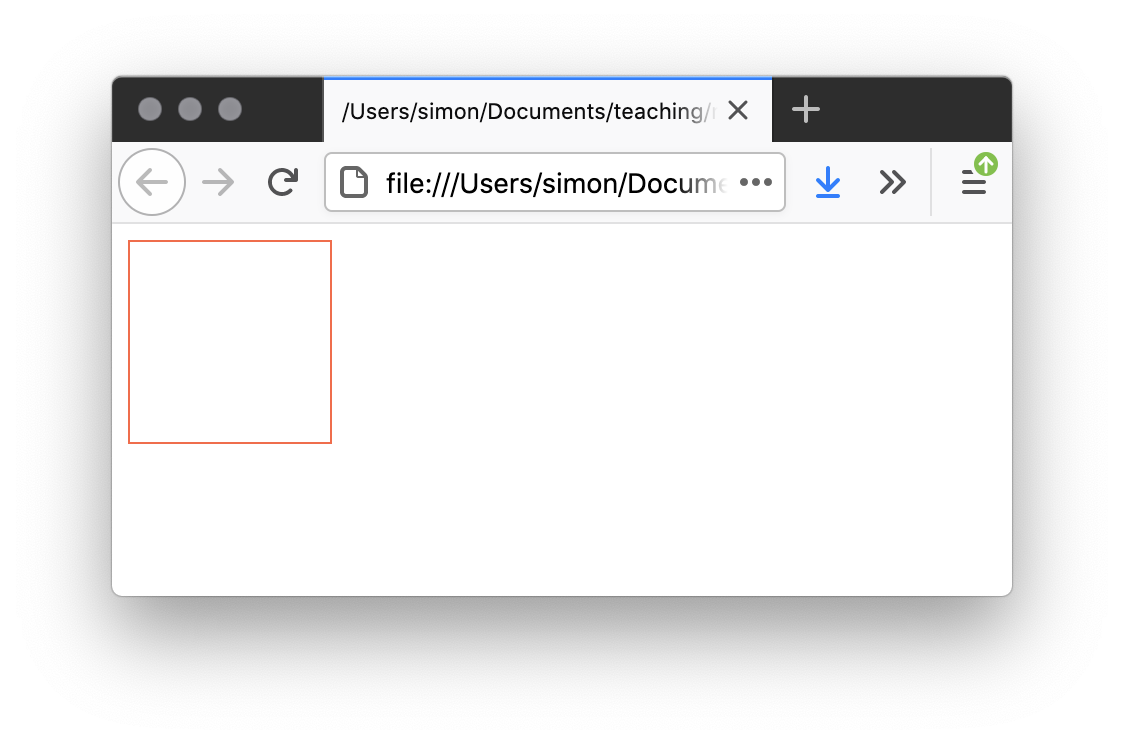
\includegraphics[width=0.8\textwidth]{figures/canvas}
\label{fig:canvas}
\caption{}
\end{figure}



\section{Drawing on our canvas}
\paragraph{} With that basic setup we can now add graphics to our page by drawing on our canvas. We need a 2D context and an alternative in case <canvas> isn’t supported:

\begin{lstlisting}
<!DOCTYPE HTML>
<html>
   <head>
      <style>
         #my_canvas{border:1px solid tomato;}
      </style>
   </head>
   
   <body>
      <canvas id = "my_canvas" width = "100" height = "100"></canvas>
      <script>
        var canvas  = document.getElementById("my_canvas");
        if (canvas.getContext) {   
            var ctx = canvas.getContext('2d');   
            // Add you drawing code here...
        } else {      
            // Do something else if user's browser doesn't
            // support the canvas element, i.e. retrieve
            // an image file as a replacement or a message
        } 
      </script>
   </body>
</html>
\end{lstlisting}

\paragraph{} Notice the script section which does three important things:

\begin{enumerate}
\item Retrieves a handle for the canvas using getElementyId()
\item Creates a 2D drawing context which we can use to actually draw onto the canvas
\item Outputs a message for the user if they are on a browser which doesn't support the canvas element (or else let's you perform an alternative function like retrieve a static image file from a server)
\end{enumerate}

\paragraph{} Our page still looks the same, like this:

\begin{figure}[H]
\centering
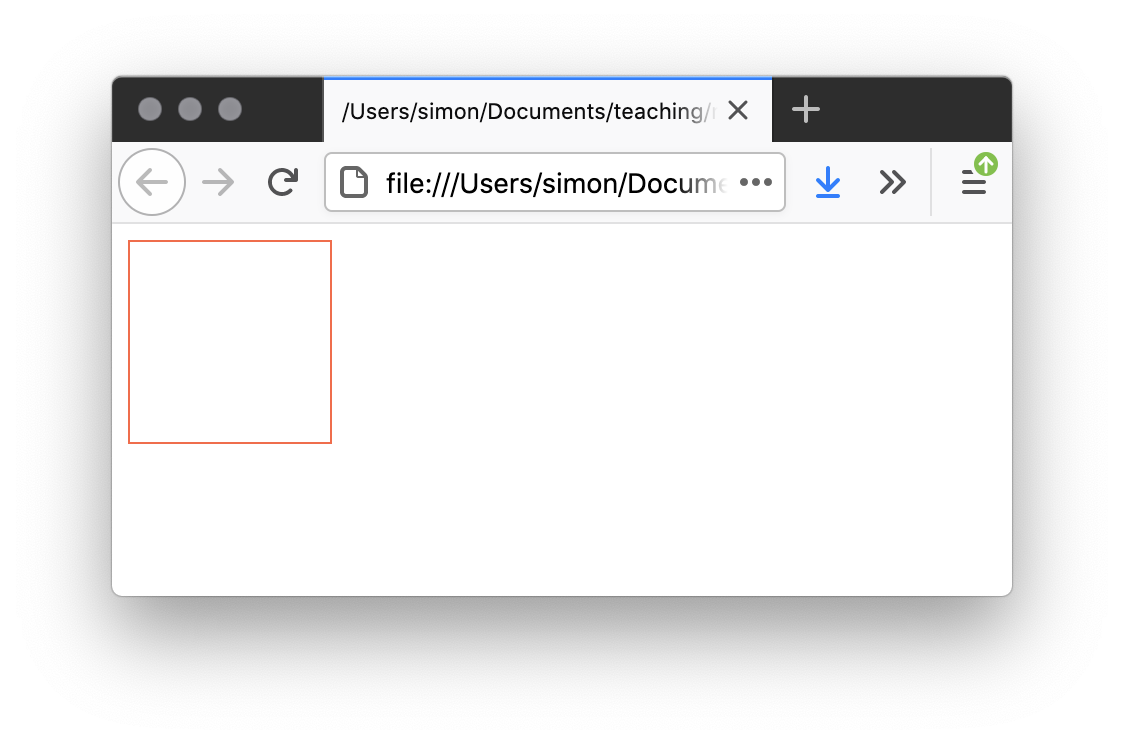
\includegraphics[width=0.8\textwidth]{figures/canvas}
\label{fig:canvas}
\caption{}
\end{figure}


\paragraph{} This is because we haven't yet actually drawn anything onto the canvas. We'll next look at three basic drawing functions we can use:

\begin{itemize}
\item Drawing Rectangles
\item Drawing Circles
\item Drawing Lines
\end{itemize}



\section{Drawing Rectangles}
\paragraph{} Drawing a rectangle is as simple as giving the starting and finishing coordinates for the upper left (starting) and lower right (finishing) corners, for example:

\begin{lstlisting}
<!DOCTYPE HTML>
<html>
   <head>
      <style>
         #my_canvas{border:1px solid tomato;}
      </style>
   </head>
   <body>
      <canvas id = "my_canvas" width=360 height=240 ></canvas>
      <script>
        var canvas  = document.getElementById("my_canvas");
        var ctx = canvas.getContext('2d');
        ctx.fillStyle = "tomato";
        ctx.fillRect(25,25,100,100);
      </script>
   </body>
</html>
\end{lstlisting}

\paragraph{} Notice that in addition to creating a filled rectangle using the fillRect() function we also set the fillStyle by setting a colour. We've also simplified the code a little for this demonstration by removing the checks on whether the context could be created. In the real world you would do these checks just in case your user had a browser that didn't support the canvas element but in order to give clarity to our examples this has now been omitted. You should expect to see something like the following as a result:

\begin{figure}[H]
\centering
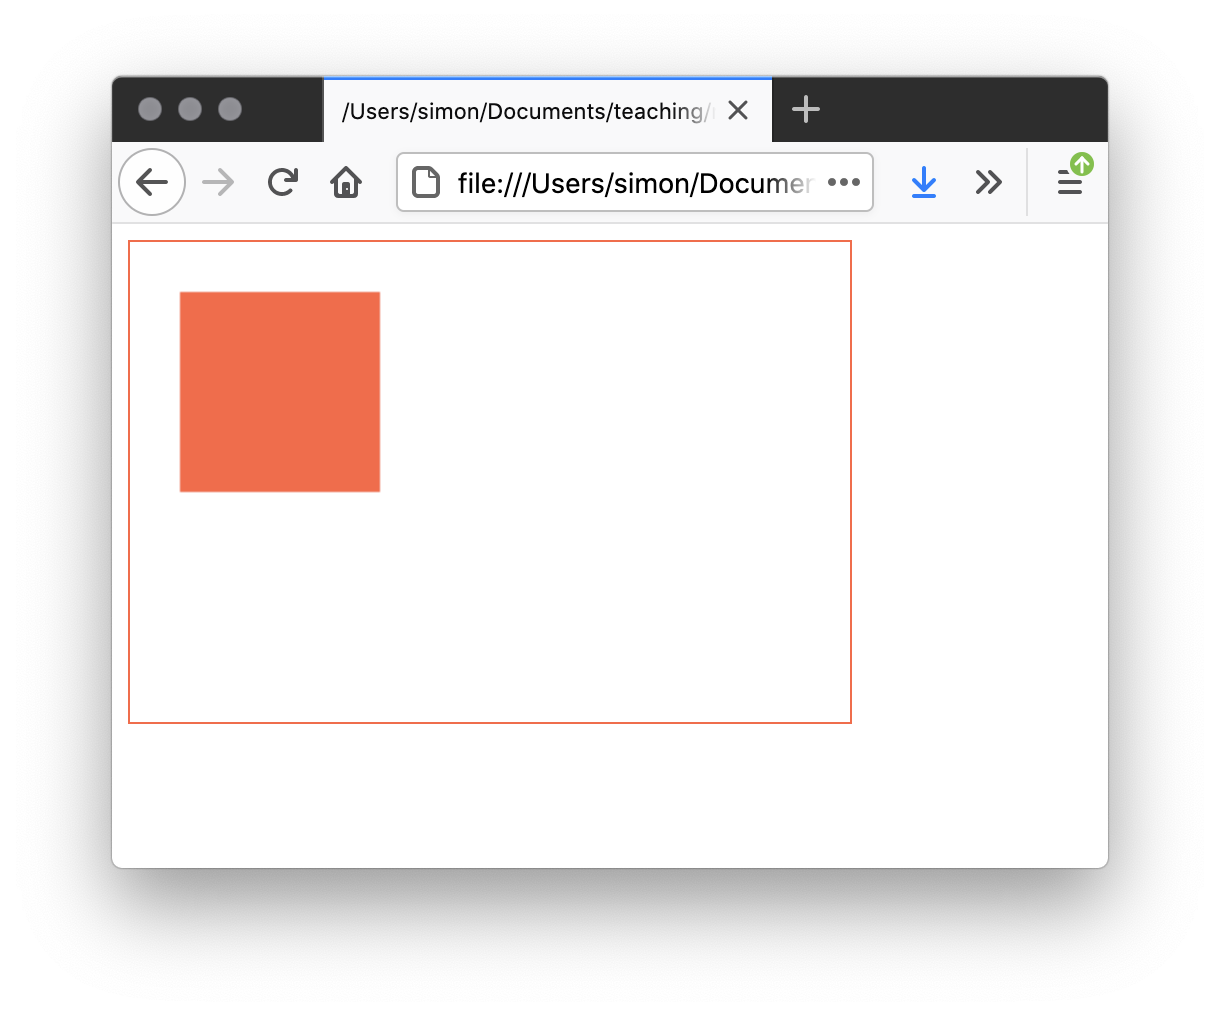
\includegraphics[width=0.8\textwidth]{figures/canvas-red-square}
\label{fig:canvas-red-square}
\caption{}
\end{figure}


\section{Drawing Circles}
\paragraph{} Drawing circles is similar to, but slightly more complex than, drawing rectangles. This is because we are actually drawing curves, or arcs, which just happen to begin and end in the same place. In the following example we've omitted the HTML boilerplate and just presented the JS code but it should drop straight into the HTML structure we previously built.

\begin{lstlisting}
 <script>
        var canvas  = document.getElementById("my_canvas");
        var ctx = canvas.getContext('2d');
        ctx.strokeStyle = "green";
        ctx.lineWidth = 1
        ctx.beginPath();
        ctx.arc(75,75,50,0,Math.PI*2,true);  
        ctx.moveTo(110,75);
        ctx.arc(75,75,35,0,Math.PI,false);   
        ctx.moveTo(65,65);
        ctx.arc(60,65,5,0,Math.PI*2,true); 
        ctx.moveTo(95,65);
        ctx.arc(90,65,5,0,Math.PI*2,true);  
        ctx.stroke();
</script>
\end{lstlisting}

\paragraph{} Notice here that we used the strokeStyle instead of fillStyle to set the colour. We've also specified a lineWidth or 1 pixel. Then we indicate that we want to create a path, the specific movement of our brush across the canvas. After that we use a series of arcs and movements (moveTo) which builds a sequence of brush strokes on the canvas, basically defining the path that we started. What is happening is that we are making a mark on the canvas by using the arc() function then lifting the brush and moving it to another location to make another mark, again using the arc() function, and so on. After we have defined all of the arcs that we want to draw then we use the stroke() function to actually make the marks onto the canvas.
\paragraph{} Note that drawing a single circle onto our canvas is actually as simple as this:

\begin{lstlisting}
var c = document.getElementById("my_canvas");
var ctx = c.getContext("2d");
ctx.beginPath();
ctx.arc(100, 75, 50, 0, 2 * Math.PI, false);
ctx.stroke();
\end{lstlisting}

\paragraph{} However our more complex example yields a slightly more interesting result:

\begin{figure}[H]
\centering
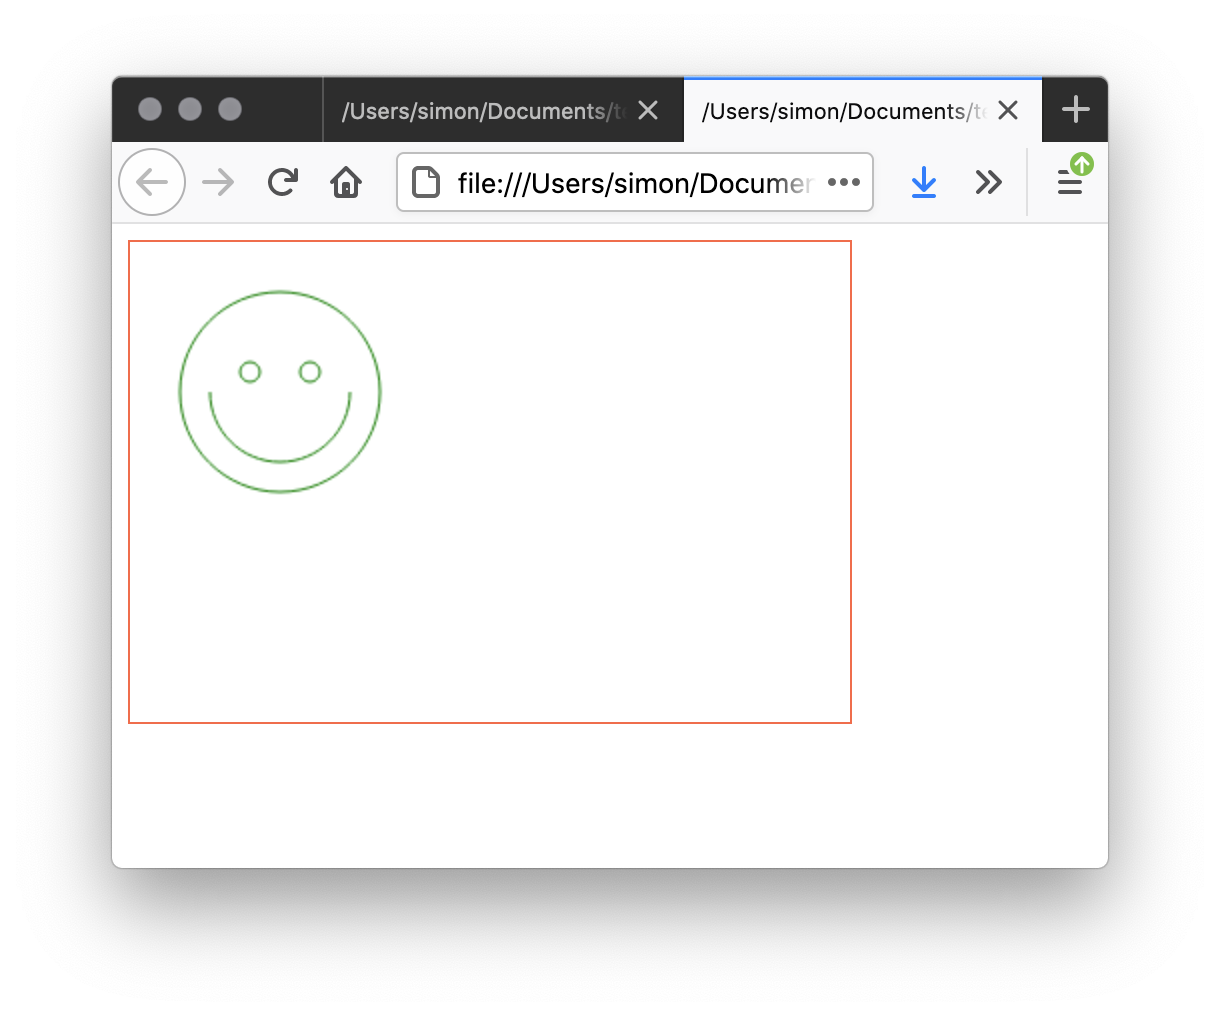
\includegraphics[width=0.8\textwidth]{figures/canvas-smiley}
\label{fig:canvas-smiley}
\caption{}
\end{figure}


\paragraph{} The arc() function parameters are as follows:

\begin{lstlisting}
context.arc(x,y,r,sAngle,eAngle,counterclockwise)
\end{lstlisting
}
\paragraph{} where x and y are the coordinates for the center of our circle, r is the radius, sAngle and rAngle are the starting and finishing angles, and counterclockwise indicates the direction in which to draw the arc. The trickiest aspect of using arcs is working out the start and finish angles relative to the centre. These are measured in radians so start at 0 and grow to 2 * pi.


\section{Drawing Lines}
\paragraph{} Finally, let's consider how to draw lines. Again the tricky part is deciding where you want your lines to start and end and determining the correct corresponding coordinates for the start and end points of our stroke.

\begin{lstlisting}
      <script>
        var canvas  = document.getElementById("my_canvas");
        var ctx = canvas.getContext('2d');
        ctx.strokeStyle = "green";
        ctx.lineWidth = 1;
        for (i=0;i<10;i++){
            ctx.lineWidth = 1+i;
            ctx.beginPath();
            ctx.moveTo(5+i*14,5);
            ctx.lineTo(5+i*14,140);
            ctx.stroke();
        }
        </script>
\end{lstlisting}

\paragraph{} This time we've include a little bit of additional JS to draw a series of lines using a for loop, so that each iteration through the loop creates a new line of increasing size. Again we're creating a path that is defined using a sequence of moveTo() and lineTo() function calls before finally calling stroke() to actually make our marks on the canvas. This is a little different to the arcs before in that we are using moveTo to specify the starting points then lineTo to move from the starting point of our line to the end point. Within both lineTo and moveTo we are merely specifying an x and y coordinate for a location on the canvas. We should see this result:

\begin{figure}[H]
\centering
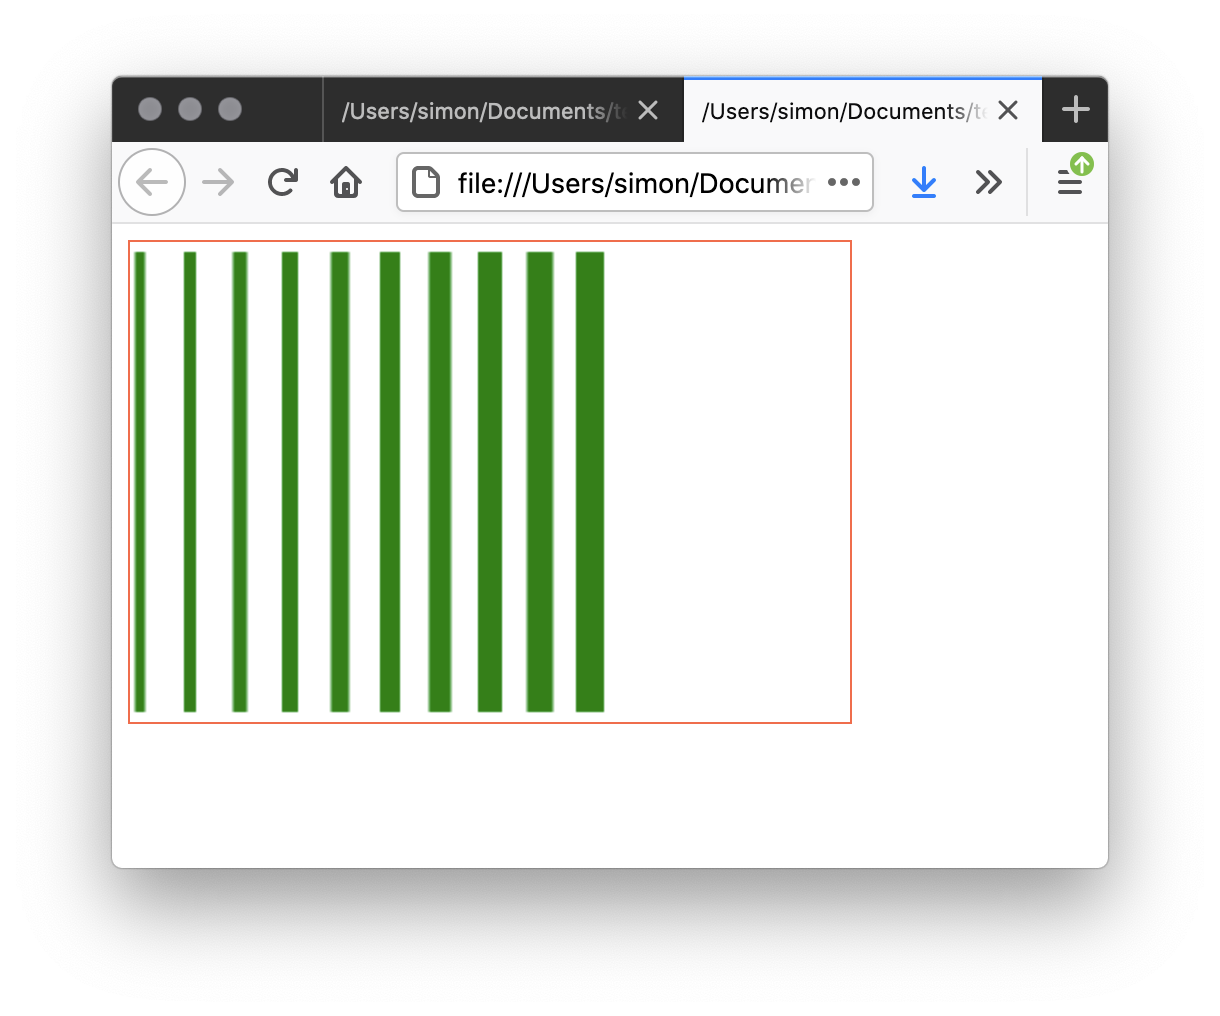
\includegraphics[width=0.8\textwidth]{figures/canvas-lines}
\label{fig:canvas-lines}
\caption{}
\end{figure}


\section{Summary}
\paragraph{} So far in this topic we've considered:

\begin{itemize}
\item How to play existing audio files on our pages
\item How to create sounds from scratch using the AudioContext, and
\item How to create 2D graphics from scratch using the HTML canvas.
\end{itemize}

\paragraph{} There is an awful lot more to both of these topics, sound and vision, each of which could be covered in an entire module, or even an entire degree programme. As a result, this unit should be considered as merely the starting point and the briefest of introductions and overviews. However, it should be sufficient to help you understand how both sound and vision fit into the context of a web document and start giving you ideas for how they can be exploited.
